\documentclass[11pt]{article}

\usepackage[margin=1in]{geometry}
\usepackage{booktabs}
\usepackage{amsmath}
\usepackage{graphicx}
\usepackage{natbib}
\usepackage[hidelinks]{hyperref}
\usepackage{microtype}
\providecommand{\Description}[1]{}

% ============================================================================
% WORKSHOP CUT (~6pp) of the P1 scheduler paper. Single argument: allocation as
% a capability-growth mechanism. The full 7-finding version is main.tex.
% Shares fig-reachability.png, fig-cost-per-grad.png, references.bib.
% ============================================================================

\title{Allocation Is a Capability-Growth Mechanism\\
in a Self-Growing LLM Red-Team}

\author{Soren Obounou Nguia\\
\small Independent researcher \quad \texttt{nguiasoren@gmail.com}}

\date{June 2026}

\begin{document}
\maketitle

\begin{abstract}
\noindent
A self-growing red-team harvests reusable attack techniques, reproduces them against deployment configurations, and graduates the effective ones into a permanent repertoire. We report that what gates this growth is not technique quality but \emph{evaluation allocation}---which harvested candidates ever get evaluated under a fixed budget. A cost-optimal greedy scheduler reproduces resisted attacks through an escalation ladder that short-circuits on the first breach; because harvested candidates sit last, they are starved---85\% of all eligible strategy-appearances never run, and the candidate-bearing tier reaches 7\% reachability. The failure is invisible in outcome logs and only became measurable once we instrumented \emph{reachability}, which separates ``evaluated and failed'' from ``never evaluated.'' Making the starved candidates reachable converts them from apparently-worthless to graduating: in a matched experiment, 3 of 3; and on a deliberately least-favourable sample of the twenty \emph{least-tried} candidates the greedy scheduler had never reached, 8 of 20 (40\%) graduate versus 0 under the identical-input greedy baseline (Fisher exact $p=0.003$). The evaluation budget is a cheap lever: cost-per-graduation \emph{falls} as more candidates are admitted---\$8.37, \$7.01, \$1.44 at $K=3,5,20$---because under an evaluation quota each ladder runs the full rotation regardless, so candidates ride a fixed cost. The claim is a reframing: in a self-growing system, allocation is a lever on \emph{capability}, not merely cost.
\end{abstract}

\section{Introduction}

Red-team research mostly measures attack effectiveness: a technique, a target, a success rate. We study the layer underneath---the orchestration that decides, under a budget, \emph{which} harvested techniques ever get evaluated. The system is a self-growing red-team that harvests reusable techniques rather than fixed prompt strings, reproduces them against deployment configurations, and promotes the ones that win a real reproduction into a repertoire it reuses.

The expectation going in was that growth would be gated by the supply and quality of techniques. It is not. It is gated by allocation, and the gate was invisible in the system's logs until we changed what we logged---from \emph{outcomes} (what ran) to \emph{opportunities} (what could have run). This short paper makes one argument along a single chain---reachable, tested, breach, graduate---and shows that a cost-optimal scheduler had silently broken its first link while every conventional log showed the system working. The fix is a small allocation change, and the result is that the change converts latent, never-evaluated candidates into permanent capability. We report the graduation \emph{rate} at $N=20$ with a significance test, and the economic behaviour of the budget lever, which is inverted from the diminishing returns most exploration systems exhibit.

\section{System: techniques, the ladder, and why candidates starve}

The unit of growth is a reusable technique---``escalate across turns,'' ``render the objective as an image''---that enters the lifecycle as a \texttt{candidate} and is promoted to \texttt{active} only when it wins a reproduction. To test whether a resisted (``EVADE-band'') attack can be broken, the system runs an \emph{escalation ladder}: $\sim$28 transform strategies across five tiers---image renderers, chain-of-jailbreak edits, structured-data injection, audio styles, and a planner-driven multi-turn tier that carries the harvested candidates---each tried in order against a panel of target models, \textbf{short-circuiting on the first breach}.

Two properties of this design starve the candidates. The ladder runs one global ordering against a multi-model panel and stops at the first breach, so it optimizes ``reach a breach cheaply,'' not ``evaluate every candidate.'' And the candidates sit \emph{last}: a cheaper transform near the front almost always breaks some model first, and the ladder halts before the candidate tier runs. The harvested candidates are therefore the most likely strategies to be starved, precisely because of where the ordering places them.

\section{Measuring opportunity, not just outcome}

The instrument that made the result measurable separates two failure modes a naive log conflates: a strategy can fail because it was \emph{evaluated and the attack did not work} (capability failure) or because it was \emph{never evaluated} (orchestration failure---most often early-stop reaching a breach before the strategy ran). Before instrumenting it, a missing attempt row was ambiguous across four realities: never eligible, starved by early-stop, ranked too low, or cut off by budget.

We log the full eligible rotation per ladder. An append-only table records, for every eligible strategy in every ladder, its rank, whether it was eligible, whether it executed, and---if not---the reason (\texttt{early\_stop} / \texttt{budget} / \texttt{no\_compatible\_config} / \texttt{not\_reached}). The trace is reconstructed post-hoc from the ladder result, so the money-spending execution path is never modified. From it, $\text{reachability} = \text{executed} \div \text{eligible}$ and $\text{starvation} = \text{early-stopped} \div \text{eligible}$ become first-class, queryable signals. This is the precondition for everything that follows: you cannot diagnose an allocation failure on a log that only records what ran.

\section{Allocation, not technique quality, gates growth}

\paragraph{The greedy scheduler starves candidates.} A greedy reorder---sort each tier by smoothed historical breach rate so the likely winner is tried first---is a \emph{correct} optimizer of its stated objective. On a 40-primitive paid sweep (greedy, no candidate quota) the median winner sat at rotation rank 0 and escalation cost \$0.35 per breach. The reachability instrument exposed the price (Figure~\ref{fig:reach}): 85\% of all eligible strategy-appearances were lost to early-stop, with per-tier reachability of 0.40 (image) down to \textbf{0.07} for the candidate-bearing planner tier. Three candidates sat at value $\approx0.50$, reachability 0.00, starvation 1.00---not weak candidates, but \emph{invisible} ones. The run produced zero graduations. The greedy scheduler had not made growth cheaper; it had optimized growth away.

\begin{figure}[t]
\centering
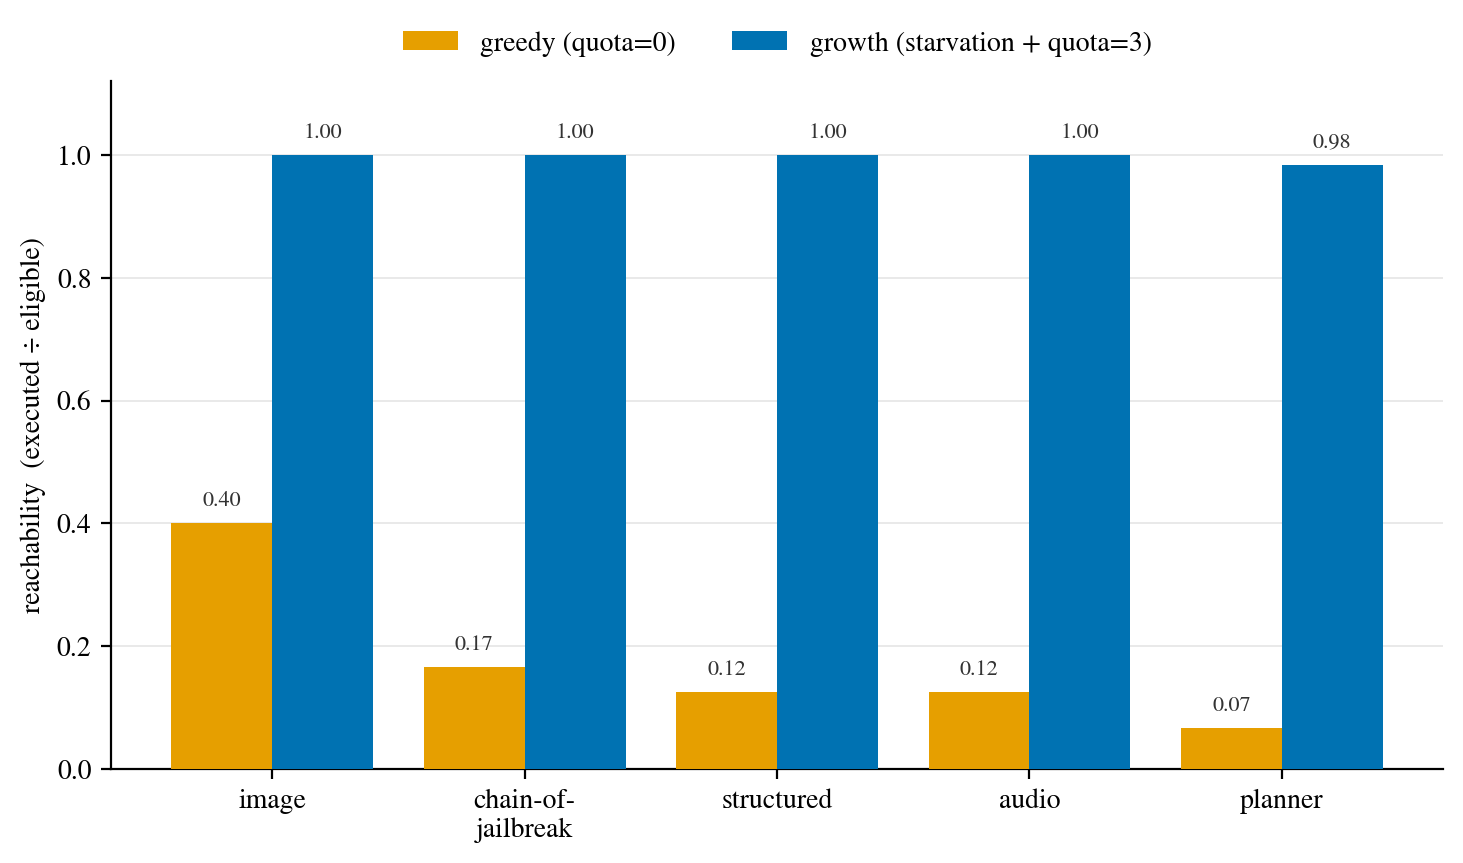
\includegraphics[width=0.68\textwidth]{fig-reachability.png}
\caption{Reachability (executed $\div$ eligible) by ladder tier, greedy vs.\ the growth configuration (starvation-aware order $+$ candidate quota). The candidate-bearing planner tier goes from 0.07 to 0.98---the starvation is in the orchestration, not the candidates.}
\Description{Grouped bar chart with five ladder tiers on the x-axis (image, coj, structured, audio, planner) and reachability from 0 to 1 on the y-axis. For each tier a short orange greedy bar sits beside a tall blue growth bar. The orange bars descend from about 0.40 at image to about 0.07 at planner, while every blue bar reaches near 1.0.}
\label{fig:reach}
\end{figure}

\paragraph{Making candidates reachable graduates them.} The question was strictly causal: if a starved candidate is made reachable, does it breach and graduate? Only running the candidates answers it. Holding the primitive set fixed and changing only the scheduler policy---starvation-aware ordering plus a candidate quota that suppresses early-stop until candidates have been attempted---drove the candidate tier from 0.07 to 0.98 reachability and overall starvation from 85\% to 1\%. In that matched experiment, all three admitted candidates breached and graduated, against zero under the identical-input greedy baseline.

\paragraph{The rate, at $N=20$.} Three is an existence proof, not a rate, and the matched experiment used candidates from the well-tried head of the pool. To measure the rate honestly we raised the selection cap to 25 and the quota to 20 so one run would evaluate twenty \emph{fresh, least-tried} candidates---the tail the greedy scheduler never reaches---against the four EVADE parents that escalate to the candidate tier. Of the twenty, \textbf{eight breached and graduated (40\%)} against the zero greedy evaluates of that set; Fisher's exact on 8/20 versus 0/20 gives two-sided $p=0.003$. The honest correction is in this number: the head-of-pool sweeps suggested $\sim$87.5\%, but the least-tried tail graduates at two in five, which is what a survivorship account predicts and what a deployment should plan around. The ``0/20'' is the established greedy-starvation baseline rather than a fresh randomized arm, and the matched contrast remains the experiment above; the larger $N$ buys a defensible rate, not a smaller $p$.

\paragraph{The budget is a cheap lever.} The selection budget $K$---how many candidates are admitted per sweep---turns out to be a dominant and economically inverted lever. Cost-per-graduation \emph{falls} as $K$ rises: \$8.37 at $K=3$, \$7.01 at $K=5$, \$1.44 at $K=20$ (Figure~\ref{fig:cost}). The cause is structural. Under an evaluation quota each ladder runs the \emph{full} rotation regardless of how many candidates are admitted, so harvested candidates ride along on a cost that is already being paid---ladder execution is a fixed cost, candidate evaluation is marginal. Raising $K$ amortizes the fixed cost over more graduations. Candidate slots were never the scarce resource; running the ladder is. The graduation yield per candidate does fall over the same range as the pool's strong head is exhausted, so the two saturation points---one defined on yield, one on dollars---do not coincide, and the dollar metric is the one that should govern how deep to sweep.

\begin{figure}[t]
\centering
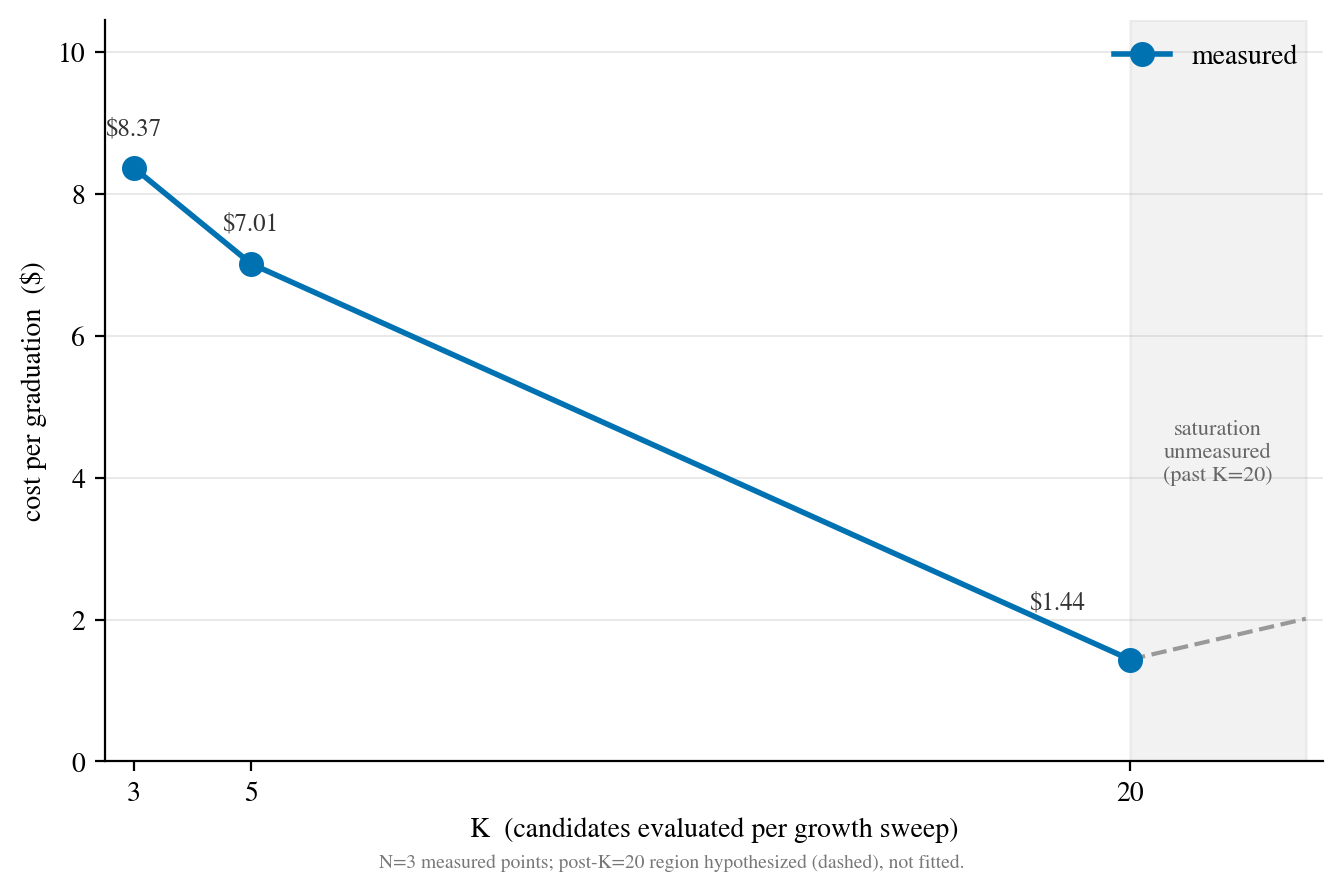
\includegraphics[width=0.62\textwidth]{fig-cost-per-grad.png}
\caption{Cost-per-graduation against $K$, three measured sweeps. It falls as $K$ rises, because the fixed full-rotation cost is amortized over more graduations.}
\Description{Line plot with K (candidates per growth sweep) on the x-axis and cost per graduation in dollars on the y-axis. Three measured points connected by a descending line drop from \$8.37 at K=3 to \$7.01 at K=5 to \$1.44 at K=20. A shaded band past K=20 is labelled saturation unmeasured, with a dashed segment extending into it.}
\label{fig:cost}
\end{figure}

\section{Limitations}

The findings are from one live system with a six-model panel; the per-system magnitudes are panel- and period-specific. The $K=3$ and $K=5$ sweeps used different candidate batches (the first graduated and left the pool), so that part is ``two growth sweeps both succeeded,'' not a controlled marginal-$K$ curve; the $K=20$ sweep is the one that measures the tail rate against a baseline. The starvation-aware \emph{ordering} operates within tiers, while the cross-tier reach into the candidate tier came from the \emph{quota}---the two are complements, and conflating them would misattribute the effect. The headline contrast is a constructed baseline (the greedy scheduler evaluates these candidates zero times by construction) checked against a matched randomized arm at small $N$, not a single large randomized trial; we state both rather than the stronger one alone.

\section{Related work}

Our contribution is orthogonal to the body of work on attack \emph{effectiveness}---which technique breaks which model. The nearest systems are the self-growing attack libraries: \citet{zhou2025autoredteamer} maintain a lifelong attack library with cost-aware selection, and \citet{liu2025autodanturbo} discover and recombine reusable strategies. We take the self-growing-repertoire idea from that line but study the orchestration underneath it---what gets evaluated, and how a fixed budget is allocated---which neither measures. Search-based attackers such as \citet{mehrotra2024treeofattacks} \emph{prune} candidate attacks to save queries; applied to an evaluation ladder that is exactly the move that produces the starvation we measure, and the value lost to non-evaluation, which we instrument, is the quantity pruning discards without recording. The multi-turn escalation framing follows Crescendo \citep{russinovich2025crescendo} and the PyRIT tooling lineage \citep{lopezmunoz2024pyrit}. A bandit formalization (Thompson sampling, contextual bandits) is the natural next step, which we defer until the measured bottleneck---budget, not ordering---is mapped, since posterior machinery on a sparse substrate would overfit.

\section{Conclusion}

A cost-optimal scheduler silently broke the first link of the chain it was meant to serve---\emph{reachable}, tested, breach, graduate---while every conventional log showed the system working. The telemetry that records what could have happened but did not is what made the break visible, and a bounded allocation change converted invisible candidates into permanent capability at a falling cost per graduation. In a self-growing system, evaluation allocation is a lever on capability, not merely on cost.

\bibliographystyle{plainnat}
\bibliography{references}

\end{document}
